%Konversi Bilangan (Arsitektur Komputer)
%Kelas : D4 TI 1B
%Khadijah Hasanah Putri Harahap 1174022
%Liyana Majdah Rahma 1174039
%Luthfi Muhammad Nabil 1174035
%Nisrina Aulia Firdaus 1174098
%Salwaa Tania 1174047
%Septia Rahayu 1174044
%Diana Satima Gistivani 1154018
\section{Konversi Bilangan}
\begin{verbatim}
Konversi bilangan adalah sebuah cara pada sistem bilangan dengan basis tertentu yang hasilnya akan dibuat menjadi bilangan dengan basis yang lainnya. 
Yaitu dengan cara membagikan bilangan yang desimal dengan dua dan kemudian diambil sisa pembagiannya.
\end{verbatim}
caranya dengan mengalikan masing-masing bit pada bilangan dengan posisi nilainya.
\\\\Didalam dunia perkomputer kita dapat mengenal empat macam-macam bilangan , seperti bilangan biner,bilangan oktal, bilangan desimal , dan yang terakhir adalah bilangan hexadesimal. Bilangan biner atau binary digit (bit) sendiri merupakan bilangan yang terdiri dari 1 dan 0. Bilangan oktal sendiri merupakan bilangan yang terdiri dari 0,1,2,3,4,5,6 dan 7.
Sedangkan bilangan desimal sendiri merupakan bilangan yang terdiri dari 0,1,2,3,4,5,6,7,8 dan 9. Dan yang terakhir adalah bilangan hexadesimal yang merupakan bilangan yang terdiri dari 0,1,2,3,4,5,6,7,8,9,A,B,C,D,E dan F.
\\\\Macam - macam Sistem Bilangan :
\begin{itemize}
\item Bilangan Biner
\item Bilangan Oktal
\item Bilangan Desimal
\item Bilangan Heksadesimal
\end{itemize}

\subsection{Bilangan Biner}
\cite{hutahaean2015konsep} Sistem bilangan biner merupakan sistem dengan penulisan angka yaitu 0 dan 1.Sistem bilangan biner modern ditemukan oleh Gittfried Wilhem Leibniz pada abad ke 17. Sistem biner juga biasa disebut dengan bit atau,Binary digit. (Hutanaen, 2015, p. 33)
\subsubsection{Konsep Bilangan Biner}
Bilangan biner menggunakan metode yang berkaitan dengan basis,bilangan biner juga menggunakan berbasis 2. Adapun contoh biner sebagai berikut : \\
\begin{equation} 1110_{2} = (1x23)+(1x22)+(1x21)+(0x20) \end{equation}\\
\begin{equation} = 8+4+2+0\end{equation}
\begin{equation}= 14 \end{equation}

\subsubsection{Konversi Sistem Bilangan Biner ke Oktal}
\begin{figure}[ht]
\centerline{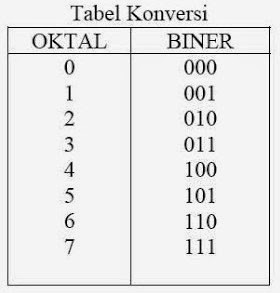
\includegraphics[width=0.4\textwidth]{figures/konversioktal.jpg}}
\caption{Tabel Konversi Bilangan Biner ke Oktal}
\label{konversioktal}
\end{figure}
\break
Cara untuk mengkonversi bilangan biner ke oktal dapat dilakukan dengan mengkonversi tiga buah digit biner. Dapat dilihat pada gambar \ref{konversioktal} untuk dapat merubah bilangan biner ke bilangan oktal, kita harus perhatikan bahwa pada setiap bilangan oktal mewakili 3 bit dari bilangan biner. Jadi, jika kita temukan bilangan biner 111110 dikonversikan ke bilangan oktal, langkah awak yang harus dilakukan adalah membagi-bagi bilangan biner tersebut, pada setiap bagian 3 bit, dapat dimulai dari sebelah Kanan ke Kiri, hingga menjadi seperti ini : 111 110 yang jika di koversikan ke dalam oktal maka hasil yang di dapat adalah 76 dalam bilangan oktal.

\subsubsection{Konversi Sistem Bilangan Biner ke Desimal}
Bilangan Biner dapat dikonversikan ke bentuk desimal dengan cara mengalikan satu-satu bilangan atau dengan dua basis biner pangkat 0 dan pangkat 1. Mengalikan bit dalam bilangan dengan position valuenya.Bilangan bineri 11001 dapat dikonversikan ke dalam bentuk desimal senilai : \\

\begin{equation}
11001_{2} = (1x20)+(0x21)+(0x22)+(1x2)+(1x22) \\
= 1+0+0+8+16 
= 25
\end{equation}

\subsubsection{Konversi Bilangan Biner ke Bilangan Hexadesimal}
Konversi bilangan biner ke bilangan hexadesimal hampir mirip seperti Konversi pada bilangan oktal. Hanya saja pada bilangan hexadesimal memakai 4 digit angka yang diambil dari bilangan biner.Selain itu untuk nilai yang lebih besar dari 9 dapat diganti dengan huruf Heksadesimal seperti A,B,C,D sampai H. 
\subsection{Bilangan Oktal}
Bilangan oktal adalah sistem bilangan yang berbasis 8 dan mempunyai delapan simbol bilangan yang berbeda : 0,1,2,...,7.
Teknik pembagian yang berurutan dapat menggunakan untuk mengubah bilangan desimal menjadi bilangan oktal. Bilangan desimal yang akan diubah secara berturut-turut dibagi dengan 8 dan sisa pembagian harus selalu dicatat. 
\subsubsection{Konversi Bilangan Oktal ke Bilangan Biner}
Cara ini merupakan kebalikan cara konversi biner ke oktal. Setiap digit oktal akan langsung dikonversi ke biner lalu hasilnya digabungkan.
\\contoh:
\\548 = …….2 ?
\\
\begin{enumerate}
\item Pertama-tama hitung 58 = 1012 (Lihat cara konversi dari desimal ke biner)
\item Lalu hitung 48 = 1002
\item Sehingga didapat 548 = 1011002
\item Anda juga dapat menggunakan rumus di ms excel OCT2BIN() yang akan menkonversi bilangan oktal ke biner
\end{enumerate}

\subsubsection{Konversi Oktal ke Desimal}
Cara untuk mengkorvesikan bilangan oktal ke heksadesimal yaitu dengan mengkonveksikan bilangan oktal tersebut ke biner terlebih dahulu kemudian bilangan tersebut di konveksikan ke heksadesimal. Untuk lebih jelasnya, perhatikan contoh konveksi bilangan oktal ke heksadesimal sebagai berikut:
\\ Contoh konversi oktal ke heksadesimal:
\begin{equation}
\\357_{8}=......_{16} 357 \end{equation}oktal sama dengan berapa bilangan heksadesimal?
Adapun cara pengerjaannya sebagai berikut adalah:
\begin{enumerate}
\item Kita pisahkan 357 menjadi 3, 5, dan 7 kemudian konversikan ke biner 
\item 3 = 011 5=101 7=111
\item Setelah dapat biner nya yaitu 011101111 kemudian konversi biner tersebut ke heksadesimal. 
\item 011101111 -------- 1111 = 15 = F 1110 = 14 = E 0 = 0
\item Maka di dapat bahwa 357 oktal sama dengan EF hexadesimal 
\end{enumerate}

\subsection{Bilangan Desimal}
Bilangan desimal adalah bilangan yang menggunakan 10 angka mulai 0 sampai 9 berturut-turut. Setelah angka 9 , maka angka berikutnya adalah 10,11,12 dan seterusnya. Bilangan desimal disebut juga dengan bilangan berbasis 10.
\subsubsection{Cara mengkoversikan bilangan desimal ke biner}
\begin{figure}[ht]
\centerline{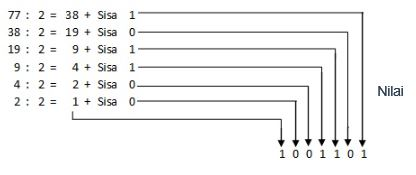
\includegraphics[width=1\textwidth]{figures/konversibiner.JPG}}
\caption{Cara mengkonversikan bilangan desimal ke biner}
\label{konversibiner}
\end{figure}
Seperti yang bisa kita lihat pada gambar \ref{konversibiner} bahwa cara mengkonversikan bilangan desimal ke dalam bilangan biner adalah dengan membagi bilangan desimal dengan nilai 2 (basis). Cara ini merupakan cara yang sering digunakan oleh banyak orang dan cara ini cukup mudah untuk di pahami dan diterapkan. Hasil yang di dapat dari perhitungan pada gambar \ref{konversibiner} adalah bilangan desimal 77 = 1001101 (bilangan biner). Dengan menggunakan rumus perhitungan konversi tersebut, kita bisa lihat langkah - langkah nya seperti berikut ini : 
\begin{enumerate}
\item Pertama kita bagi 77 dengan 2, didapat bilangan bulat hasil bagi adalah 39 dengan sisa hasil bagi adalah 1,atau dengan kata lain 77=2*(36+1)
\item Selanjutnya bilangan bulat hasil bagi tersebut (36) kita bagi dengan 2 lagi, 36/2=18,sisa hasil bagi 0
\item Ulangi lagi langkah tersebut sampai bilngan bulat hasil bagi sama dengan 0. Setelah itu tulis sisa hasil bagi mulai dari bawah ke atas
\item Barulah kita mendapatkan hasil bahwa bilangan desimal 77 adalah bilangan desimal dari bilangan biner 1001110.
\end{enumerate}

\subsubsection{Cara mengkonversikan bilangan desimal ke oktal}
Dengan menggunakan rumus yang mirip dengan biner kita bisa lakukan juga untuk bilangan berbasis 8(oktal).
\\Langkah - langkah :
\begin{enumerate}
\item Pertama-tama 67/8=8, sisa 3
\item Lalu 8/8=0,sisa 0
\item Terakhir 1/8=0 sisa 1
\item Dengan demikian dari hasil perhitungan di dapatkan 6710=1038
\item Konversi dapat menggunakan fungsi pada aplikasi microsoft excel DEC20CT() untuk konversi bilangan desimal ke oktal.
\end{enumerate}

\subsubsection{Konversi bilngan desimal ke heksadesimal}
Seprti halnya biner dan oktal,kita pun akan menggunakan teknik perhitungana yang sama.\\

Langkah-langkah:
\begin{enumerate}

\item Pertama-tama 67/16=4, sisa 3
\item Lalu 4/16=0, sisa 4
\item Dengan demikian dari hasil pehitungan di dapatkan 6710=4316
\end{enumerate}

\subsection{Bilangan Heksadesimal}
Heksadesimal adalah sistem bilangan berbasis 16 yang menggunakan 16 jenis simbol. Simbol yang digunakan adalah 10 digit bilangan angka yaitu 0, 1, 2, 3, 4, 5, 6, 7, 8, dan 9 ditambah dengan 6 simbol huruf yaitu huruf A hingga F. Dimana A = 10, B = 11, C= 12, D = 13 , E = 14 dan F = 15.
\subsubsection{Konversi Bilangan Heksadesimal ke Biner}
\begin{figure}[ht]
\centerline{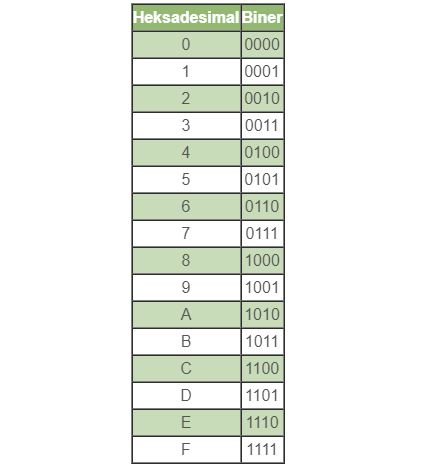
\includegraphics[width=0.5\textwidth]{figures/konversiheksa.JPG}}
\caption{Tabel Konversi Bilangan Heksadesimal ke Biner}
\label{heksakebiner}
\end{figure}
Berbeda dengan sistem bilangan desimal, bisa di lihat pada \ref{heksakebiner} simbol yang digunakan dari sistem ini menggunakan 16 buah simbol, mulai dari 0 sampai 9, kemudian dilanjut dari A sampai F. Jadi, angka A sampai F merupakan simbol untuk 10 sampai 15. Contoh penulisan : C516.
Untuk dapat mengetahui bagaimana cara mengubahnya antara bilangan satu dengan yang lain. Sebenarnya pada dasarnya, bilangan heksadesimal digunakan sebagai salah satu cara untuk menampilkan informasi bilangan biner dalam deret yang lebih pendek.

\subsubsection{Konversi bilangan Heksadesimal ke Oktal}
Untuk konversi pada Bilangan Heksadesimal ke Oktal memiliki proses yang sama dengan cara konversi Bilangan Oktal ke Desimal. Terlebih dahulu lakukan konversi bilangan heksadesimal ke biner lalu Konversi dari bilangan biner ke bilangan Oktal
\begin{equation}
\\Contoh : F5_{16} = ...._{8}
\end{equation}
\begin{enumerate}
\item Konversi bilangan Heksadesimal menjadi biner \begin{equation}F5_{16} = 1111 0101_{2}\end{equation}
\item Kemudian kelompokkan bilangan biner tersebut setiap digit dimulai dari yang paling kanan
\item Selanjutnya 3 digit bilangan biner tersebut dikonversikan ke oktal
\end{enumerate}

\subsubsection{Konversi bilangan Heksadesimal ke Desimal}
Pada Konversi Heksadesimal ke desimal dapat mengalikan digit bilangan Heksadesimal dengan pangkat 16 dari kanan ke kiri mulai dengan pangkat 0,1,2....,seterusnya
\begin{equation}
\\Contoh : F5_{16} = ......_{10} ? 
\end{equation}
\break 
\begin{equation}
F5_{16} = (15 \times 16_{1})(10) + (5 \times 16_{0})(10) = 240 + 5 = 245
\end{equation}
\section{Fungsi dari Konversi Bilangan}
Membuat sebuah program tidak hanya membutuhkan bahasa pemrograman. Pada bagian komputernya juga memerlukan sebuah bahasa yang dimengerti oleh komputer tersebut. yaitu bilangan biner. jadi salah satu Fungsi dari konversi bilangan ini salah satunya adalah untuk membuat sebuah program. Selain memakai sebuah sistem bilangan desimal, pembuatan sebuah program itu terkadang juga menggunakan bilangan biner, oktal, dan hexadesimal.
Fungsi lain dari Konversi bilangan ini salah satunya adalah untuk membaca sebuah perintah yang dimana perintah tersebut masih menggunakan perintah yang hanya bisa dibaca oleh komputer yaitu Biner. tetapi dengan adanya Konversi Bilangan, Sebuah angka tersebut bisa dijadikan sebagai suatu line perintah bahkan sebuah kata yang nantinya dapat dimunculkan oleh komputer kepada pengguna. Pembuatan aplikasi sendiri membutuhkan sebuah Konversi Bilangan yang nantinya akan menggerakan sebuah modul - modul dalam sebuah perangkat yang dipakai dalam aplikasi tersebut. 
Konversi Sendiri dilakukan dalam sebuah Processor atau ALU yang mereka hanya dapat membaca kode biner yang nantinya saat setelah diproses akan dimasukan ke memori yang nanti akan dikonversi ditampilkan ke layar dengan berbentuk yang sesuai dengan yang dibutuhkan \cite{noersasongko1996mengrnal}
\\Membuat sebuah program tidak hanya membutuhkan bahasa pemrograman. Pada bagian komputernya juga memerlukan sebuah bahasa yang dimengerti oleh komputer tersebut. yaitu bilangan biner. jadi salah satu Fungsi dari konversi bilangan ini salah satunya adalah untuk membuat sebuah program. 
\\Fungsi lain dari Konversi bilangan ini salah satunya adalah untuk membaca sebuah perintah yang dimana perintah tersebut masih menggunakan perintah yang hanya bisa dibaca oleh komputer yaitu Biner. tetapi dengan adanya Konversi Bilangan, Sebuah angka tersebut bisa dijadikan sebagai suatu line perintah bahkan sebuah kata yang nantinya dapat dimunculkan oleh komputer kepada pengguna. Pembuatan aplikasi sendiri membutuhkan sebuah Konversi Bilangan yang nantinya akan menggerakan sebuah modul - modul dalam sebuah perangkat yang dipakai dalam aplikasi tersebut. 

\section{Penerapan Konversi Bilangan}
Konversi Bilangan diterapkan khususnya pada bidang Teknologi. Selain sebagai instruksi, Konversi sendiri dapat dikenal sebagai pengenal dalam situasi tertentu. seperti untuk mengenal warna dan sebagainya. Beberapa contoh dari penerapan tersebut adalah sebagai berikut : 
\begin{itemize}
\item Sebagai kode warna dalam pemrograman \\ Konversi Bilangan sering sekali dipakai untuk mengetahui berapa tingkat warna dan seberapa pekat warna tersebut. Konversi Bilangan pada kasus ini menggunakan Konversi Desimal ke Heksadesimal dimana warna terbagi menjadi Merah, Hijau, Biru. 
\item Sebagai Penampil Angka dalam Kalkulator \\ Dengan adanya Konversi Bilangan, Angka yang dikirimkan ke memori akan diubah kedalam bentuk angka biner yang sebelumnya dikonversi dengan menekan sebuah tombol yang mengirimkan aliran kepada memori untuk mengirimkan angka biner.
\item Untuk menampilkan hasil perhitungan dari ALU \\ Pada ALU, Bilangan yang dipakai adalah bilangan Biner yang sangat kecil memungkinkan untuk dibaca oleh computer atau monitor pada umumnya. Oleh karena itu, Untuk menampilkan hasil dari perhitungan, Dibutuhkan sebuah konversi yang dilakukan setelah proses perhitungan mengeluarkan sebuah hasil yang nanti akan ditampilkan oleh Monitor.
\end{itemize}

\section{Rangkuman}
Konversi Bilangan adalah Konversi dimana sebuah bilangan akan dikonversikan menjadi tipe bilangan yang lain. Tipe bilangan sendiri cukup beragam, seperti Bilangan Biner, Desimal, Oktal, dan Heksadesimal. Cara pengonversiannya sendiri bermacam ? macam, ada yang mampu langsung dikonversikan menjadi bilangan tipe tujuan atau diubah terlebih dahulu ke bilangan decimal. Pemakaian dari Konversi Bilangan pun beragam. Dimulai dari proses hitungan pada kalkulator dan ALU sampai pembacaan kode pada kode Heksadesimal di computer. 
\\Pada dasarnya Konversi bilangan memiliki beberapa fungsi baik dalam Komputer maupun diluar computer. Dengan adanya metode ini kita diharapkan dapat membaca dan mengkonversi sebuah instruksi kedalam computer yang dapat terbaca oleh computer lalu dapat dikonversikan ke dalam bentuk sebuah bilangan yang kita inginkan. Bahkan seseorang yang buta warna dapat melihat warna yang tidak bisa dia lihat dengan kode yang telah tersedia yaitu kode warna. 
\break
\break
\break
%\begin{itemize}
%\item Definisi dari Konversi Bilangan didapatkan dari sebuah artikel dengan judul "APLIKASI PEMBELAJARAN KONVERSI BILANGAN MENGGUNAKAN METODE COMPUTER ASSISTED INSTRUCTION (CAI)" \cite{gulo2016aplikasi}
%\item Metode Konversi Bilangan didapatkan dari sebuah buku berjudul "Konsep Sistem Informasi" \cite{hutahaean2015konsep}
%\item Penerapan Konversi Bilangan didapatkan dari sebuah buku dengan judul "Mengenal Dunia Komputer" \cite{noersasongko1996mengrnal}
%\end{itemize}